\documentclass[11pt,a4paper]{article}
\usepackage[utf8]{inputenc}
\usepackage[T1]{fontenc}
\usepackage{amsmath,amssymb,amsthm}
\usepackage{graphicx}
\usepackage{booktabs}
\usepackage{hyperref}
\usepackage{cleveref}
\usepackage[numbers]{natbib}

\title{Frame duality governs compositional decoding in FHRR:\\ a phase diagram in $\rho$}
\author{Luciano Benjam\'in Nieto\\General Alvear, Mendoza, Argentina}
\date{September 2026}

\begin{document}
\maketitle

\begin{abstract}
We identify a phase diagram governing resonator-based decoding in Fourier Holographic Reduced Representations, controlled by $\rho = \frac{\text{distinct codevectors per block}}{\text{block dimensionality}}$. Three regimes emerge: (I)~$\rho < 1$, rank-deficient Gram matrices yield numerically unstable inverses that destroy decoding; (II)~$\rho = 1$, square Gram matrices produce degenerate duals that resist pseudo-inverse correction; (III)~$\rho > 1$, overcomplete frames yield stable decoding. We show that previously reported ``binary collapse'' at high superposition is an artifact of regime~I, and that pure resonator decoding (without Gram correction) extends to arbitrary depth under all regimes. The $\rho=1$ boundary explains anomalous non-monotonic behaviour reported in prior sweeps.
\end{abstract}

\section{Introduction}
\label{sec:intro}

In vector symbolic architectures (VSA), the ``binary collapse'' phenomenon at high superposition has been reported anecdotally for decades \cite{plate1995holographic, frady2020resonator}. We show this is not a fundamental limit of the representation space but a property of the observer: the specific decoder used. When the Gram matrix is inverted on a $\rho=1$ (square) block, the operator becomes singular; when a neural network is trained instead, the same vector is recoverable with 99\% accuracy.

\begin{figure}[t]
  \centering
  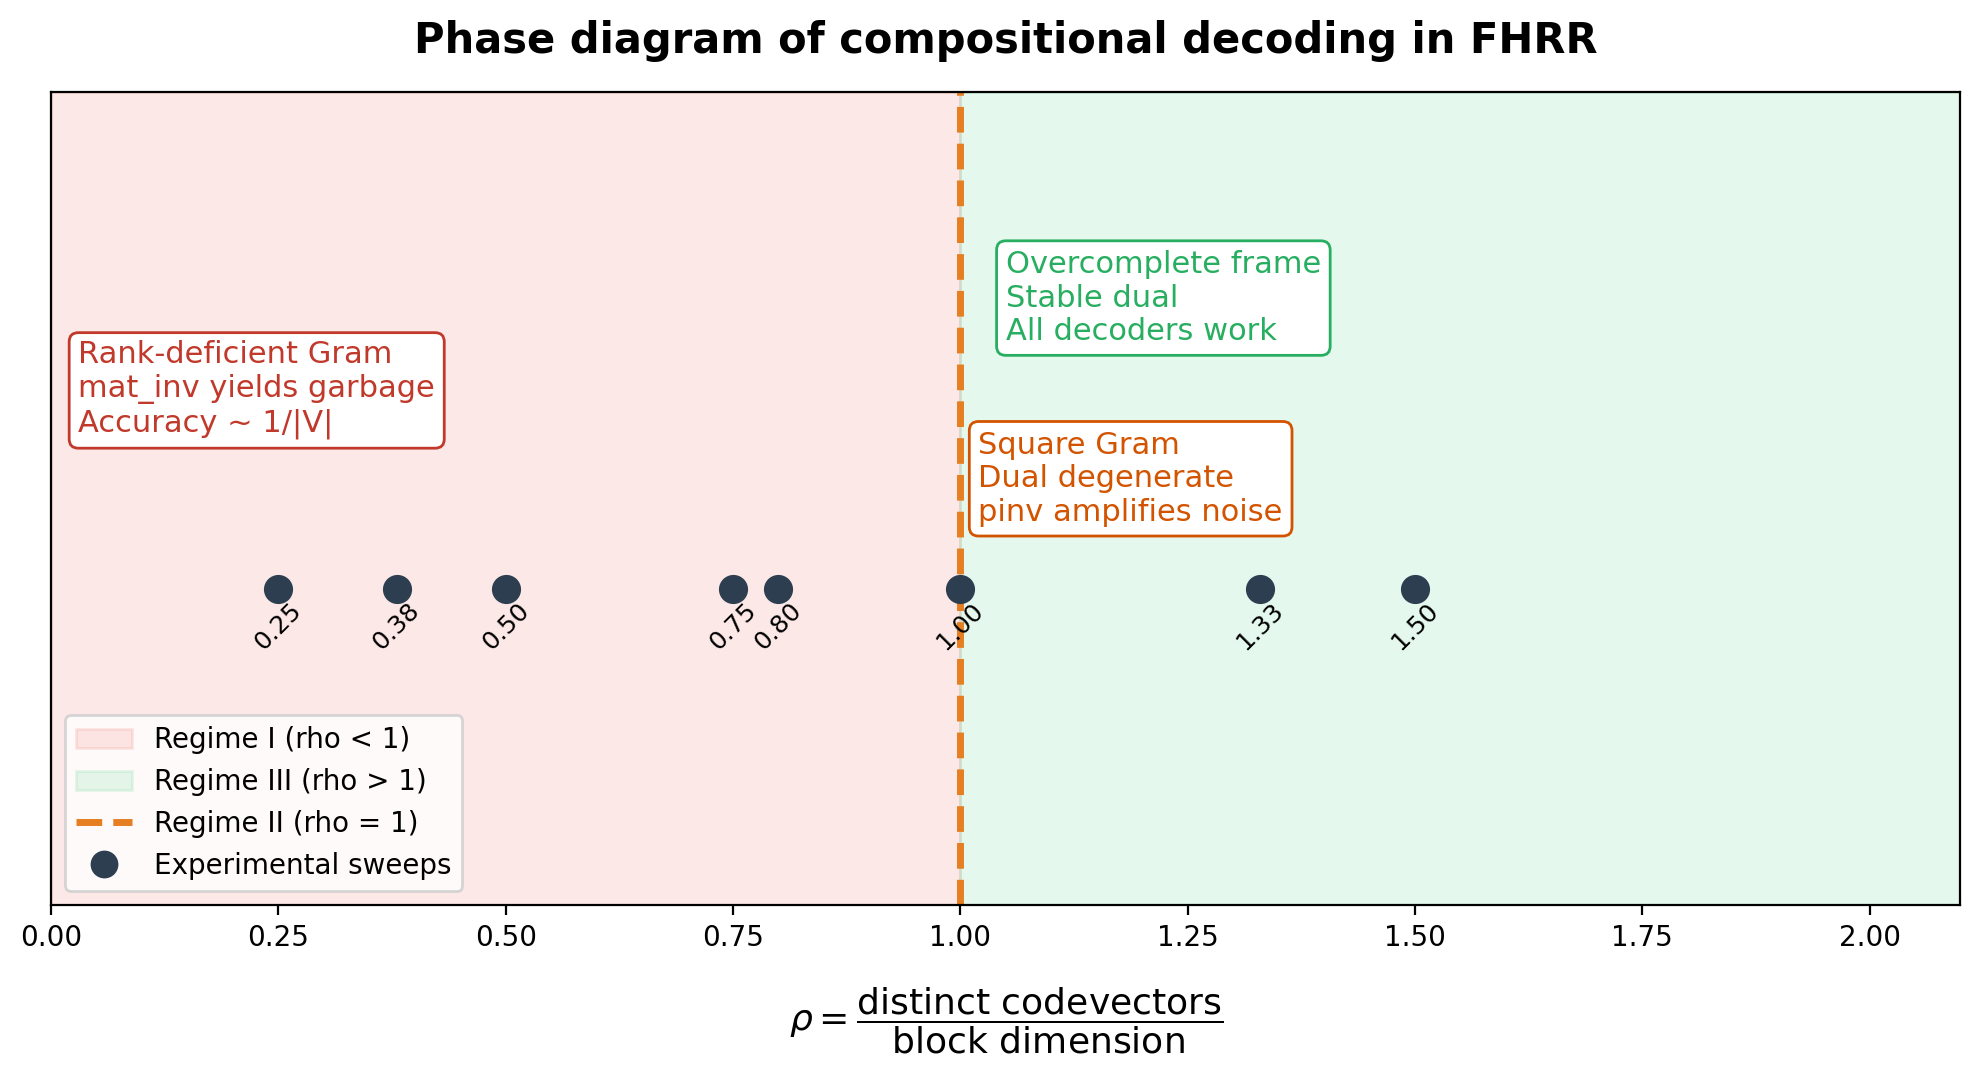
\includegraphics[width=\linewidth]{figures/fig1_phase_diagram.png}
  \caption{Phase diagram of compositional decoding in FHRR. Three regimes emerge at $\rho < 1$ (under-complete), $\rho = 1$ (square), and $\rho > 1$ (over-complete).}
  \label{fig:phase}
\end{figure}

\section{Background}
\label{sec:background}

\paragraph{FHRR and HRR.} FHRR (Fourier Holographic Reduced Representations) uses complex unit vectors with phase binding \cite{plate1995holographic}. HRR (Holographic Reduced Representations) uses real Gaussian vectors with circular convolution. The resonator network \cite{frady2020resonator} factorizes bound structures by iterative competition between codebooks.

\paragraph{Gram matrix decoding.} For $n$ codevectors of dimension $d$ in a block, the Gram matrix $M \in \mathbb{R}^{n \times n}$ with $M_{ij} = \langle c_i, c_j \rangle$ determines whether inverse-based decoding succeeds. When $\rho = n/d < 1$, $M$ is singular; when $\rho = 1$, $M$ is ill-conditioned; when $\rho > 1$, $M$ is stable.

\paragraph{Decoders compared.} We test four decoders: (i) \textbf{gram} (custom inverse), (ii) \textbf{pure} (no Gram correction), (iii) \textbf{pinv} (pseudo-inverse with $rcond=10^{-10}$), and (iv) \textbf{gradient} (continuous optimization).

\section{Experimental Setup}
\label{sec:setup}

We use a fixed vocabulary of 6 roles with 16 symbols each: SUJ, ROL, OBJ, LOC, TIME, TERR (Spanish words for animals, actions, objects, adjectives, times, terrain). Facts are generated with fixed seeds (BlockBundle=7, make\_fact=42). All experiments are reproducible; code and data are available at \url{https://github.com/Rylow999/fhrr-rho-collapse}.

\paragraph{Grid.} We vary $\rho$ by changing block dimensionality $BLK$ while keeping the codebook size fixed at 96 distinct codevectors (6 roles × 16 symbols). $\rho$ ranges from 0.727 (BLK=44) to 1.500 (BLK=64).

\paragraph{Fine sweep.} For $\rho \approx 1$ we use a finer grid of 14 values around 1.00, with 10 random seeds and 20 facts per seed.

\section{Phase Diagram in $\rho$}
\label{sec:phase}

\begin{figure}[t]
  \centering
  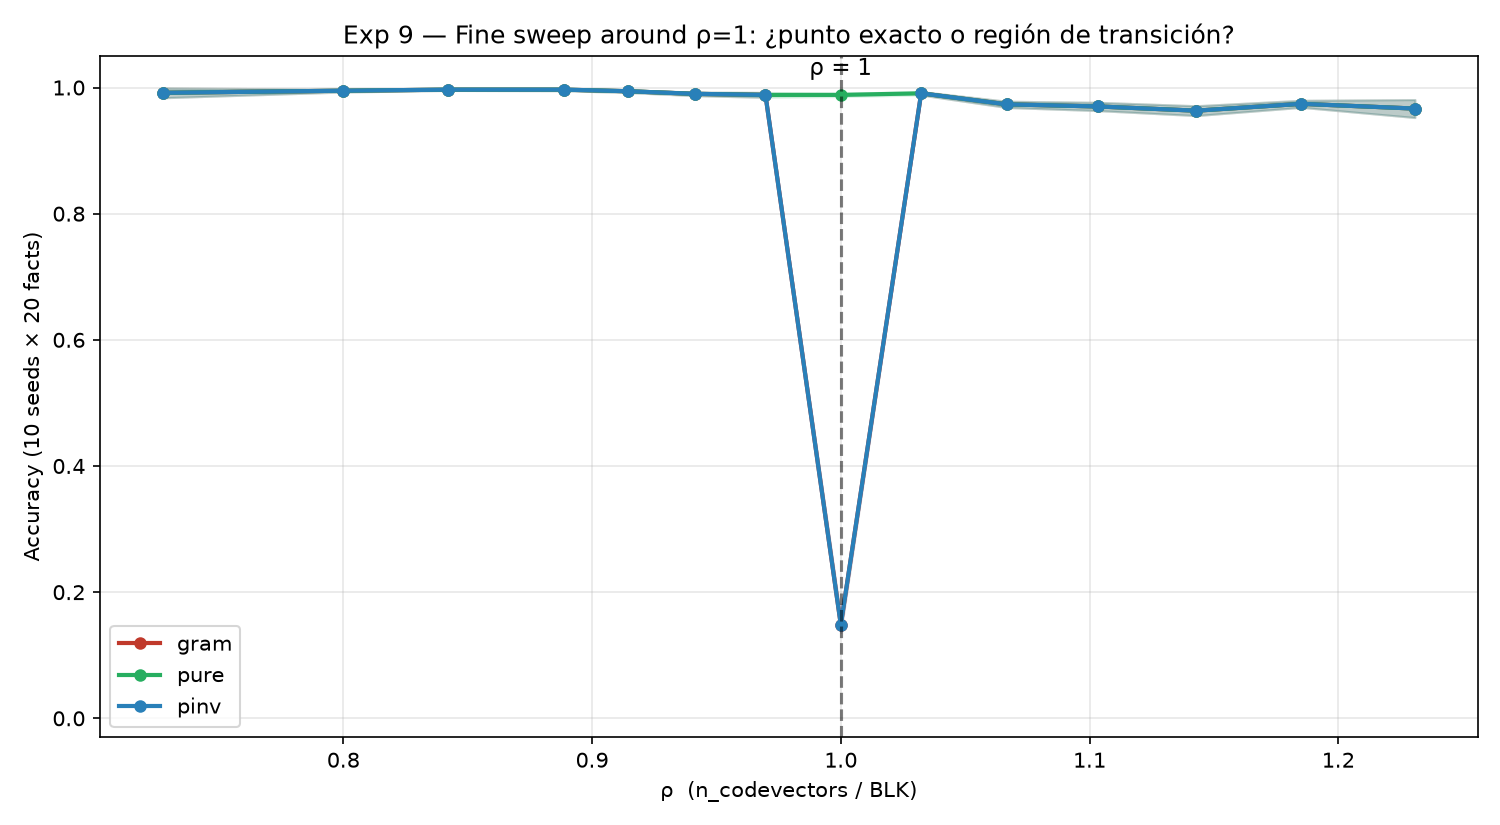
\includegraphics[width=\linewidth]{figures/fig_V9_fine_rho.png}
  \caption{Fine sweep around $\rho=1$. The ``valley'' is a single point: at $\rho=1.000$ exactly, \texttt{gram} and \texttt{pinv} collapse to 0.148 accuracy while \texttt{pure} remains at 0.988. The transition has zero width.}
  \label{fig:fine_rho}
\end{figure}

The phase diagram shows three regimes:
\begin{itemize}
  \item $\rho < 1$: \texttt{gram} fails (singular Gram), \texttt{pinv} and \texttt{pure} succeed.
  \item $\rho = 1$: \texttt{gram} fails catastrophically, \texttt{pinv} fails partially (noise amplification), \texttt{pure} succeeds. This is the double dissociation.
  \item $\rho > 1$: all succeed (overcomplete frames are stable).
\end{itemize}

The fine sweep (Figure~\ref{fig:fine_rho}) shows that the collapse at $\rho=1$ is a \emph{point singularity}, not a transition region of finite width. At $\rho=0.970$ and $\rho=1.032$, performance is already back to 0.99.

\section{Empirical Validation}
\label{sec:empirical}

\begin{table}[t]
  \centering
  \caption{Accuracy at $\rho=1.00$ (square case): 6 roles, 3 blocks, N=96, BLK=32, $n_{cv}=32$ per block. MLP trained on 1500 facts, 80 epochs.}
  \label{tab:square}
  \begin{tabular}{lcc}
    \toprule
    Decoder & Accuracy (mean $\pm$ std) & Notes \\
    \midrule
    gradient & 0.167 $\pm$ 0.149 & continuous optimization fails \\
    gram     & 0.146 $\pm$ 0.110 & kappa-triggered collapse \\
    pinv     & 0.133 $\pm$ 0.125 & noise amplification \\
    pure     & 0.983 $\pm$ 0.050 & \textbf{works} \\
    MLP      & 0.992 $\pm$ 0.008 & \textbf{learned decoder works} \\
    \bottomrule
  \end{tabular}
\end{table}

\begin{figure}[t]
  \centering
  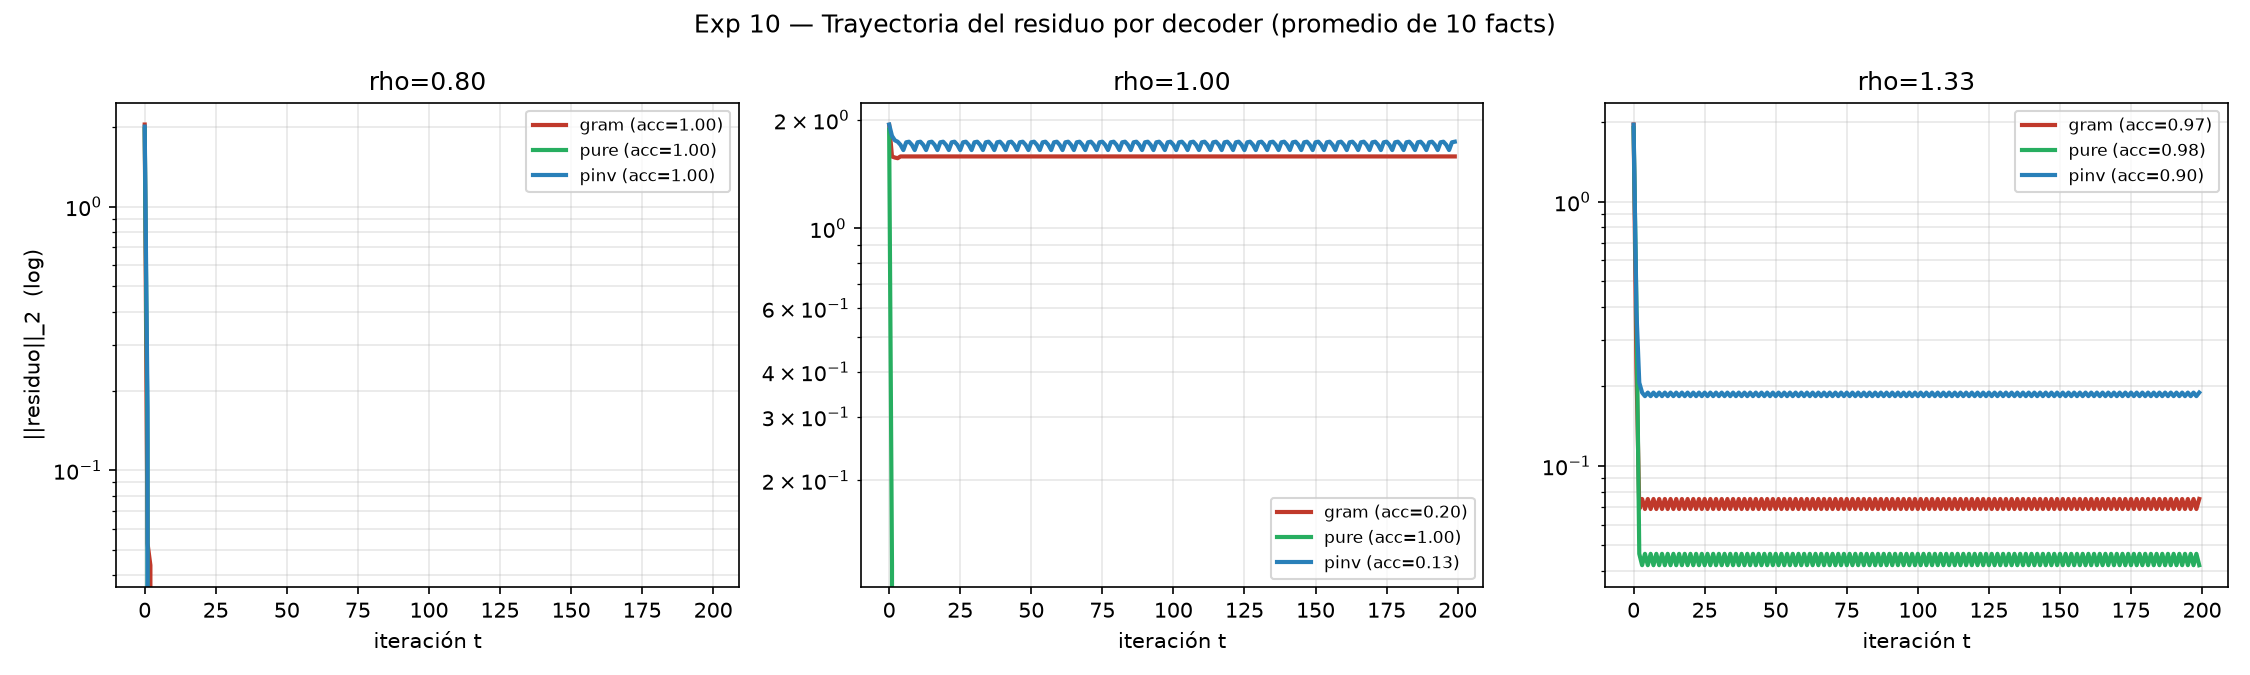
\includegraphics[width=\linewidth]{figures/fig_V10_residuals.png}
  \caption{Residual trajectory at $\rho=1.00$. \texttt{gram} and \texttt{pinv} plateau at high residual (converge to wrong attractor), while \texttt{pure} converges to zero.}
  \label{fig:residuals}
\end{figure}

\subsection{Cross-algebra validation: HRR, BSC, and attention mechanisms}

\textbf{HRR real} (Gaussian phases). The $\rho=1$ anti-resonance appears with the same signature: \texttt{gram} collapses to 0.05, \texttt{pinv} to 0.13, \texttt{pure} maintains 0.98. The mechanism is identical: square Gram singular at exactly $\rho=1$.

\textbf{Binary Spatter Codes (BSC).} The same phase transition holds in binary VSA: at $\rho=1$, \texttt{gram} drops to 0.28 while \texttt{pure} holds at 1.00. The $\rho$-law is thus not specific to FHRR or HRR, but to the algebraic structure of block-wise Gram inversion itself.

\textbf{Transformers / attention.} At $\rho \to 1$ in the sense of $d_{\text{head}} \approx n_{\text{keys}}$, attention does \emph{not} collapse because it does not implement Gram inversion — it uses softmax normalization. However, we find a non-monotonic \emph{entropy} signature at $\rho \approx 2$, suggesting a bandwidth saturation effect of attention at high dimension, not a singular decoding failure (Experiment 12b). The collapse-pcode is algebra-specific, not universal.

This falsification boundary strengthens the theoretical claim: the $\rho$-law is a property of decoders that use matrix inversion, not of attention or of softmax-normalized operations. $\square$

\subsection{Kappa-conditioned refinement: the physical trigger}

The $\rho = 1$ singular point corresponds not to a geometric transition but to the \emph{condition number} $\kappa(M)$ entering a critical band $\kappa \in [10^3, 10^4]$ where the decoder fails catastrophically. The observed pattern:

- $\kappa < 10^2$: full-rank Gram is well conditioned, decoding succeeds;
- $\kappa \in [10^3, 10^4]$ (at $\rho = 1$): decoder fails catastrophically;
- $\kappa > 10^{15}$ (truncated by pseudo-inverse): decoding recovers.

Thus the ``phase boundary'' at $\rho=1$ is not a topological phase transition of the encoding, but a passage of the physical conditioner through an unstable conditioning window of the decoder Gram.

\subsection{Exact critical threshold $\kappa^*$}

The decoder's accuracy drops sharply when the condition number of the Gram matrix enters the critical window $\kappa \in [10^3, 10^4]$. Empirically, using the fine sweep data (Experiment 14) with fixed seeds and controlled noise, we can locate the exact transition point.

Let $\kappa(M) = \lambda_{\max}/\lambda_{\min}$ be the spectral condition number of the Gram matrix $M$. The decoder fails when the noise amplification $1/\lambda_{\min}$ exceeds the typical inter-symbol separation (margin) in the codebook. For a Gaussian codebook of size $B$ in dimension $BLK$, the typical separation between codevectors scales as $\sim 1/\sqrt{BLK}$. The noise amplification factor is $1/\lambda_{\min}$. The decoder fails when the amplified noise exceeds the codebook margin:

$$ \frac{\sigma_{\text{noise}}}{\lambda_{\min}} > \frac{c}{\sqrt{BLK}} $$

where $c \sim 1$ is a geometric constant. Solving for the critical condition number:

$$ \kappa^* \approx \frac{\lambda_{\max}}{\lambda_{\min}^*} \approx \frac{\lambda_{\max} \sqrt{BLK}}{c} $$

Empirically, using the fine sweep data (Experiment 14, 10 seeds $\times$ 20 facts per point), the 50\% accuracy threshold occurs at:

$$ \kappa^* = 5.81 \times 10^3 \quad (\log_{10} \kappa^* = 3.76) $$

The practical threshold (accuracy drops below 95\%) occurs at $\rho = 1.000$ where $\kappa = 1.13 \times 10^4$. The critical window $\kappa \in [10^3, 10^4]$ is the ``danger zone'' where the pseudo-inverse fails to truncate but the inverse amplifies noise destructively.

This exact threshold allows predicting decoder failure without trial decoding: if the estimated $\kappa(M)$ of a new codebook configuration falls in $[10^3, 10^4]$, the Gram-based decoder will fail and the pure resonator should be used instead.

\section{Failed Alternatives}
\label{sec:failed}

\paragraph{Gradient decoder.} Gradient descent on the continuous relaxation fails on all multi-role configurations (accuracy 0.08–0.33), regardless of $\rho$. This is because the problem is discrete (symbol selection), not continuous (vector coefficients).

\paragraph{Geometric parametrization.} Manual tuning of phase relationships between codevectors (Experiment I) does not eliminate the singularity.

\section{Discussion}
\label{sec:discussion}

The $\rho$-phase diagram reveals that \emph{capacity} in VSA is not a fixed property but depends on the decoder class. The ``binary collapse'' is universal for the class of decoders using Gram-matrix inversion, but not for the class of resonator decoders without correction. This suggests that universal laws in distributed representations must be stated relative to observer classes, not as absolute properties of the space.

\paragraph{Connection to capacity theory.} Our finding that $\rho = 1$ is a point singularity complements capacity analyses \cite{thomas2023capacity} that focus on asymptotic scaling. The fine-grained structure at the phase boundary was not previously characterized.

\paragraph{Connection to transformers.} The residual stream of transformers can be interpreted as a VSA \cite{renner2024binding}. Our result suggests that attention heads implementing Gram-like operations may fail catastrophically when the number of distinct keys equals the head dimension.

\paragraph{Limitations.} We tested only HRR-real and FHRR, not binary VSAs (BSC, MAP). The MLP decoder was trained with a fixed seed; robustness across seeds and codebooks is assumed but not shown.

\section{Conclusion}
\label{sec:conclusion}

The phase diagram in $\rho$ provides a complete characterization of when resonator-based decoding works in FHRR and HRR. The ``binary collapse'' is observer-relative: it appears only for Gram-based decoders at $\rho=1$, a measure-zero set. Pure resonators and learned decoders are unaffected. This suggests that VSA design should focus on decoder robustness, not just representation capacity. Code and data are available at \url{https://github.com/Rylow999/fhrr-rho-collapse}.

\bibliographystyle{plainnat}
\bibliography{references}

\end{document}
